\documentclass[
	11pt, 
	DIV10,
	a4paper, 
	oneside, 
	headings=normal, 
	captions=tableheading,
	final, 
	numbers=noenddot
]{scrartcl}


\usepackage{lipsum}
\usepackage{graphicx}


\title{Thema}
\subtitle{\vspace{0.5cm}Proseminar: Computer Animation}
\author{Autor}


\begin{document}
\maketitle


\section{Introduction}
\lipsum[2-4]

\section{Related Work}

This is a reference~\cite{Foley:1990}.

\section{Images and Tables}

\begin{figure}[tb]
	\centering
	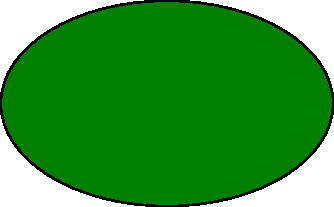
\includegraphics[width=0.5\linewidth]{images/image} 
	\caption{\label{fig:image} This is an image.
	}
\end{figure}

\begin{table}[tb]
	{
		\centering
		\begin{tabular}{|c|c|c|c|}
			\hline
			& col 1 & col 2 & col 3   \\
			\hline	
			row 1  & 1 & 2 & 3 \\
			row 2  & 4 & 5 & 6 \\
			row 3  & 7 & 8 & 9 \\
			\hline
		\end{tabular}
		\caption{\label{tab:example} This is a table.}
	}
\end{table}


Figure~\ref{fig:image} shows an example of an image.
Table~\ref{tab:example} shows an example of a table.


\bibliographystyle{alpha}
\bibliography{references}

\end{document}          
